\documentclass[tikz,border=8pt]{standalone}
% Shared look for every TikZ diagram. Load with % Shared look for every TikZ diagram. Load with % Shared look for every TikZ diagram. Load with \input{../../tools/tikz-style.tex}
\usepackage[T1]{fontenc}
\usepackage{lmodern}
\renewcommand{\sfdefault}{lmr}  % diagrams use the same serif as the text
\usetikzlibrary{arrows.meta, positioning, shapes.geometric, calc, fit, backgrounds}
\definecolor{cblue}{HTML}{4C78A8}
\definecolor{corange}{HTML}{F58518}
\definecolor{cgreen}{HTML}{54A24B}
\definecolor{cred}{HTML}{E45756}
\definecolor{cpurple}{HTML}{B279A2}
\definecolor{cgrey}{HTML}{6B6B6B}
\tikzset{
  every picture/.style={font=\sffamily, line width=1.2pt},
  box/.style={draw=#1, fill=#1!12, rounded corners=4pt, align=center, inner sep=7pt, minimum height=1.1cm},
  box/.default=cgrey,
  arrow/.style={-{Stealth[length=3mm]}, draw=cgrey, line width=1.4pt},
  title/.style={font=\sffamily\bfseries\Large},
  note/.style={font=\sffamily\small, text=cgrey, align=center},
}
\AtBeginDocument{\hyphenpenalty=10000 \exhyphenpenalty=10000}

\usepackage[T1]{fontenc}
\usepackage{lmodern}
\renewcommand{\sfdefault}{lmr}  % diagrams use the same serif as the text
\usetikzlibrary{arrows.meta, positioning, shapes.geometric, calc, fit, backgrounds}
\definecolor{cblue}{HTML}{4C78A8}
\definecolor{corange}{HTML}{F58518}
\definecolor{cgreen}{HTML}{54A24B}
\definecolor{cred}{HTML}{E45756}
\definecolor{cpurple}{HTML}{B279A2}
\definecolor{cgrey}{HTML}{6B6B6B}
\tikzset{
  every picture/.style={font=\sffamily, line width=1.2pt},
  box/.style={draw=#1, fill=#1!12, rounded corners=4pt, align=center, inner sep=7pt, minimum height=1.1cm},
  box/.default=cgrey,
  arrow/.style={-{Stealth[length=3mm]}, draw=cgrey, line width=1.4pt},
  title/.style={font=\sffamily\bfseries\Large},
  note/.style={font=\sffamily\small, text=cgrey, align=center},
}
\AtBeginDocument{\hyphenpenalty=10000 \exhyphenpenalty=10000}

\usepackage[T1]{fontenc}
\usepackage{lmodern}
\renewcommand{\sfdefault}{lmr}  % diagrams use the same serif as the text
\usetikzlibrary{arrows.meta, positioning, shapes.geometric, calc, fit, backgrounds}
\definecolor{cblue}{HTML}{4C78A8}
\definecolor{corange}{HTML}{F58518}
\definecolor{cgreen}{HTML}{54A24B}
\definecolor{cred}{HTML}{E45756}
\definecolor{cpurple}{HTML}{B279A2}
\definecolor{cgrey}{HTML}{6B6B6B}
\tikzset{
  every picture/.style={font=\sffamily, line width=1.2pt},
  box/.style={draw=#1, fill=#1!12, rounded corners=4pt, align=center, inner sep=7pt, minimum height=1.1cm},
  box/.default=cgrey,
  arrow/.style={-{Stealth[length=3mm]}, draw=cgrey, line width=1.4pt},
  title/.style={font=\sffamily\bfseries\Large},
  note/.style={font=\sffamily\small, text=cgrey, align=center},
}
\AtBeginDocument{\hyphenpenalty=10000 \exhyphenpenalty=10000}

\begin{document}
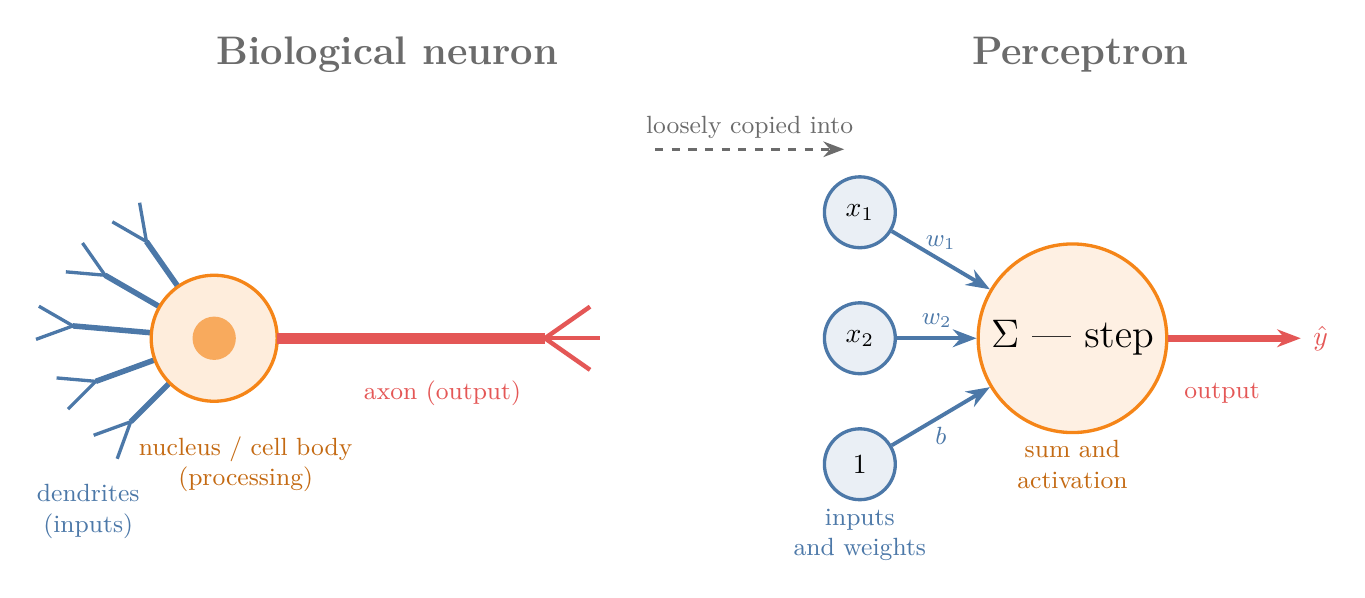
\begin{tikzpicture}
  % biological neuron
  \node[title, cgrey] at (2.2,3.6) {Biological neuron};
  \foreach \a/\l in {150/1.6, 175/1.8, 200/1.6, 225/1.5, 125/1.5} {
    \draw[cblue, line width=2pt] (0,0) -- (\a:\l) coordinate (d);
    \draw[cblue, line width=1.2pt] (d) -- ++(\a+25:0.5);
    \draw[cblue, line width=1.2pt] (d) -- ++(\a-25:0.5);
  }
  \node[circle, draw=corange, fill=corange!15, minimum size=1.6cm] (cell) at (0,0) {};
  \node[circle, fill=corange!70, minimum size=0.55cm] at (0,0) {};
  \draw[cred, line width=4pt] (0.8,0) -- (4.2,0);
  \foreach \a in {-35,0,35} \draw[cred, line width=1.6pt] (4.2,0) -- ++(\a:0.7);
  \node[note, cblue] at (-1.6,-2.2) {dendrites\\(inputs)};
  \node[note, corange!80!black] at (0.4,-1.6) {nucleus / cell body\\(processing)};
  \node[note, cred] at (2.9,-0.7) {axon (output)};
  % perceptron
  \begin{scope}[xshift=9.4cm]
  \node[title, cgrey] at (1.6,3.6) {Perceptron};
  \tikzset{inp/.style={circle, draw=cblue, fill=cblue!12, minimum size=0.9cm}}
  \node[inp] (a) at (-1.2,1.6) {$x_1$};
  \node[inp] (b) at (-1.2,0) {$x_2$};
  \node[inp] (c) at (-1.2,-1.6) {$1$};
  \node[circle, draw=corange, fill=corange!12, minimum size=1.4cm, font=\Large] (s) at (1.5,0) {$\Sigma$ | step};
  \draw[arrow, cblue] (a) -- node[above, font=\small] {$w_1$} (s);
  \draw[arrow, cblue] (b) -- node[above, font=\small] {$w_2$} (s);
  \draw[arrow, cblue] (c) -- node[below, font=\small] {$b$} (s);
  \draw[arrow, cred, line width=2.5pt] (s) -- (4.4,0) node[right] {$\hat{y}$};
  \node[note, cblue] at (-1.2,-2.5) {inputs\\and weights};
  \node[note, corange!80!black] at (1.5,-1.6) {sum and\\activation};
  \node[note, cred] at (3.4,-0.7) {output};
  \end{scope}
  \draw[dashed, cgrey, line width=1pt, -{Stealth}] (5.6,2.4) -- node[above, note] {loosely copied into} (8.0,2.4);
\end{tikzpicture}
\end{document}
